\documentclass[12pt]{article}

\usepackage{graphicx}
\usepackage{float}

\begin{document}
\title{\textbf{Café del Campo} \\Sparktech}
\maketitle

\section{Team members}
\begin{itemize}
\item Miguel Rodriguez
\item Shao-Wen Chang
\item Asadujaman Nur
\item Vincent Obigwe
\end{itemize}

\section{Introduction}

According to legend, an Ethiopian Goatherd first discovered the coffee in the 9th century. When he noticed his flock became so active and energetic after consuming some kind of Barry. Later on, he tried the same berry by himself and noticed he could stay awake longer without getting tired because of the presence of caffeine in the berry.  When the local monk witnessed this phenomenon they were intrigued and started to boil the bean and drink the water so that they could pray for a longer time even in the night thus the first coffee was born.

Later on due to colonisation in 1640 coffee was imported into Europe by Dutch merchants. After that, various coffees started to emerge. It got huge popularity, it even replaced wine and beer during breakfast since people started to notice drinking a cup of coffee boosted their productivity. Fast forward to the modern era, our life got even busier and therefore to keep our focus and energy we often drink coffee, from homemade to vending machines. Coffee is one of the most consumed and accessible drink 2nd after water. Moreover, there is no sign of decreasing its popularity. Due to its huge popularity, there are various versions of coffee and various ways to serve.

During the Hardware Engineering Lab we are going to Design and build a prototype of a Coffee vending machine Named “Café del campo” Using FPGA and VHDL. Using “VHDL”, we can program our Feature circuits, Logic, and other necessary components from scratch. For the VHDL programming, we are going to use ModelSim software. After programming our features in VHDL, we need to build the necessary circuits so that we can manufacture them. To Design and build our necessary “FPGA” PCB board we are going to Use “Eagle”. To realize our project these two methods are crucial because of the reason above. We are also going to implement some other methods  like “block diagram, Agile project management, various technologies, VHDL Implementation, PCB Design” etc. which we will discuss in detail later on in the paper.


\section{Concept Description}

A Coffee machine that provides coffees with high quality coffee. According to the type of coffee, the ratio of water, coffee powder, milk or sugar is adjusted. To acquire the desired coffee, press a number for coffee type and another for whether sugar is added. The output will then be water, coffee powder, milk and sugar if selected.

In Figure \ref{fig:espresso} we have a guide on the different combinations of coffee, streamed milk, foamed milk, water and chocolate, depending on the type of coffee that the user can possibly select

\begin{figure}[!h]
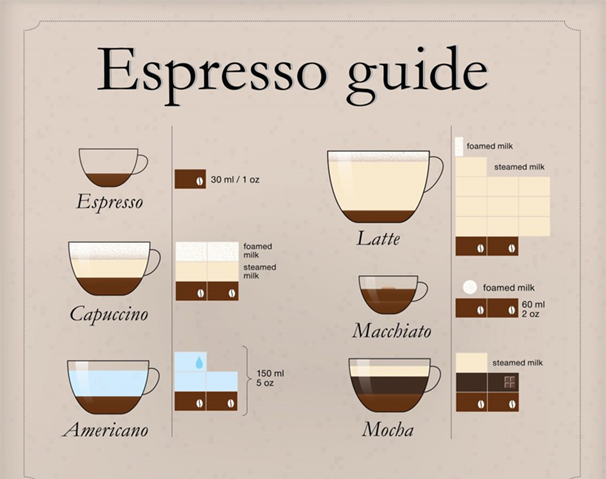
\includegraphics[scale=0.83]{imgs/expesoguide.png}
\caption{Espresso guide}
\label{fig:espresso}
\end{figure}

The block diagram of the coffee machine is described on Figure \ref{fig:block}. There will be two inputs at the beginning of the project: coffee number and sugar selection, there will be a clock or timer that will determinate when the different ingredients will be poured into the cup and on the right side, there are four outputs, coffee, water, foamed milk and streamed milk and sugar. Depending on the time and the complexity of the task there are two extra components that can be added, the cash input and the cash change.

\begin{figure}[h]
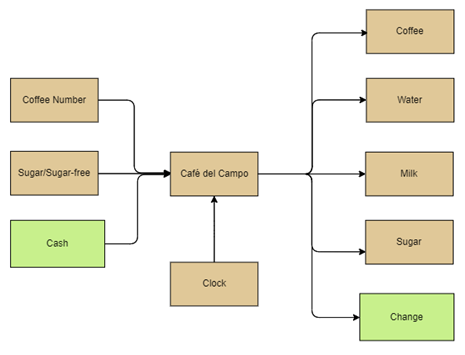
\includegraphics[scale=1.1]{imgs/blockd.png}
\caption{Espresso guide}
\label{fig:block}
\end{figure}

\section{Project / Team management}

In carrying out our project, we consider project management as an important aspect that helps us in realizing the goal and objective faster. Project management benign the application of various methods, skill knowledge and experience to achieve a detailed object that has already been set and marked as the project acceptance benchmark. It is also very important that time and budget are considered. As students we embarked on this project with the focus on managing time and delivering the best result given the limited amount of time that and the no budget we deal with.  Having this in mind, we decided to approach the whole project using the agile project management \cite{APM1}. 

Agile project management is known as an iterative means of delivering a project throughout a given life cycle. There life cycle are made up of several iterations that are all geared towards the completion of the project. This leads to us having weekly meetings to analyze tasks and evaluate progress. With Agile project management, continuous improvement and development is the goal, to enable the project to get better on further iterations. While using Agile project management, we made use of Kanban framework to be able to achieve our project \cite{APM}. 

Kanban is a framework on agile project management that is deals with growth changes and the need for continuous process improvement. The core practices involved in using Kanban are: 

1.	Visualization of tasks in a board like manner with tools such as excel. 

2.	Reduction of work in project by introducing changes incrementally 

3.	Management of the flow of to-dos

4.	Defining processes and tasks clearly

5.	Enhancing the process of feedback to enable improvement of the system.

6.	Improving workflow all together. 

To be able to properly visualize our tasks and clearly see what each member of the group has to do, we made use of GitHub projects. GitHub projects can be seen as a customizable spreadsheet that helps us integrate tasks with GitHub in our repository. It empowers more customization by enabling filtering; sorting, grouping and working with GitHUb pull requests. It further looks static with the addition of colors to determine the various stage each task is \cite{kanvanize}.


\section{Technologies}

\subsection{VHDL}

One of the technologies that we will use for this project is VHDL a hardware description language \cite{vhdl}. This language can model the behaviour of a digital system in different levels of abstraction \cite{vhdl}

\subsection{FPGA}

Field programmable gate arrays popularly known as FPGA are increasingly used to power electronic devices. A complex control algorithm can easily be implemented using FPGA for any given electronic system. Xilinx-ISE is a platform that is used for a variety of reasons depending on one’s usecase. However, it is predominantly used in relation to FPGA development. It can be used to write VHDL code and feed it into the FPGA \cite{fpga}. Xilinx-ISE is been used by us for the development of FPGA.

\subsection{EAGLE}

Eagle: According to \cite{eagle} Eagle is an electronic design automation application with schematic capture, printed circuit board layout, auto-router, and Computer-Aided Manufacturing features. EAGLE stands for Easily Applicable Graphical Layout Editor which is developed by CAD-Soft Computer GmbH. The company was acquired by Autodesk Inc in 2016. This is one of the most used software because of its basic free license which one can use for its study and personal purposes. In this course, we were advised to use eagle to represent our project which will be explained later on in PCB Design.

\section{Implementation}

\subsection{VHDL}

The VHDL code in out project is divided in three parts. The first one will take the input from the user, input is given by 6 options the first five stand respectively for Espresso, Americano, Cappucino, Late, Macchiato and the last one represents sugar. Moreover, it takes input of a clock to synchronize the system. The first module will take the user input and will organize it into a simple four-bit vector for the ten types of coffees and then outputs it. This output will be the input of the second module. Figures \ref{fig:table1} and \ref{fig:vhdl1}.


\begin{figure}[H]
\centering{ 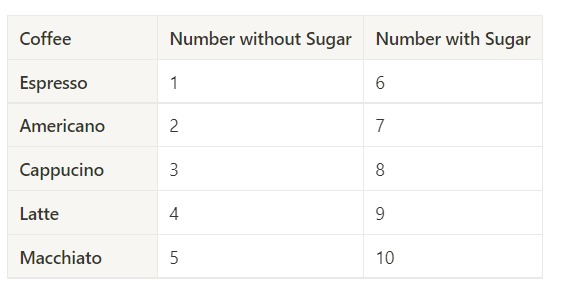
\includegraphics[scale=0.72]{imgs/table1}}
\caption{Coffee options}
\label{fig:table1}
\end{figure}

\begin{figure}[H]
\centering{ 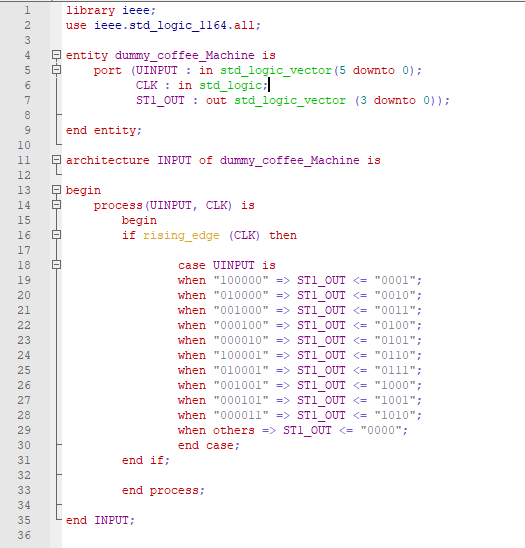
\includegraphics[scale=0.77]{imgs/vhdl1}}
\caption{First VHDL module}
\label{fig:vhdl1}
\end{figure}

The second module will take the output of the first module as an input, and will output five four-bit vectors, this vectors will represent the signal with the units that have to be poured for each case, giving a zero as an output when there is not unit that have to be poured, or up to 8, for example the units for the Latte. Figure \ref{fig:vhdl2}

\begin{figure}[H]
\centering{ 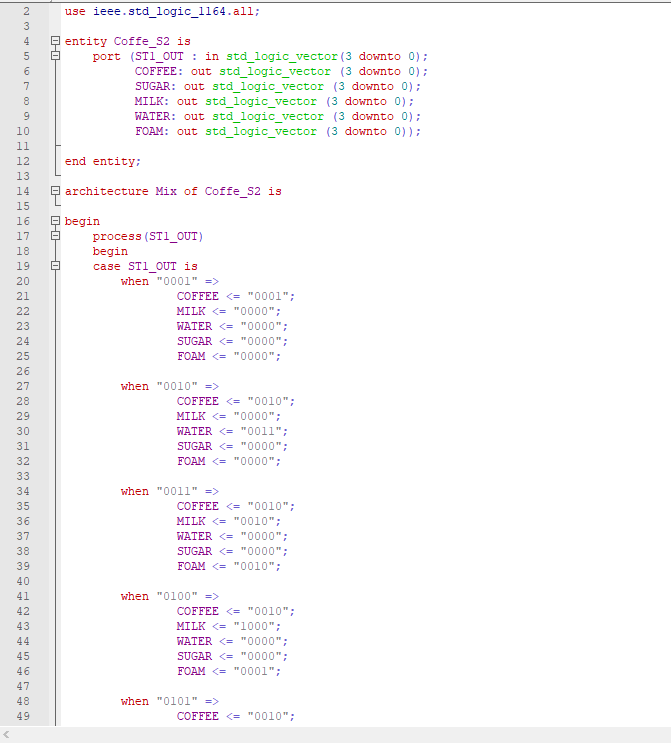
\includegraphics[scale=0.77]{imgs/vhdl2}}
\caption{Second VHDL module}
\label{fig:vhdl2}
\end{figure}

The third module combine the two previous models in one simple model. This module is the global representation of the coffee machine. Figure \ref{fig:vhdl3}



\begin{figure}[H]
\centering{ 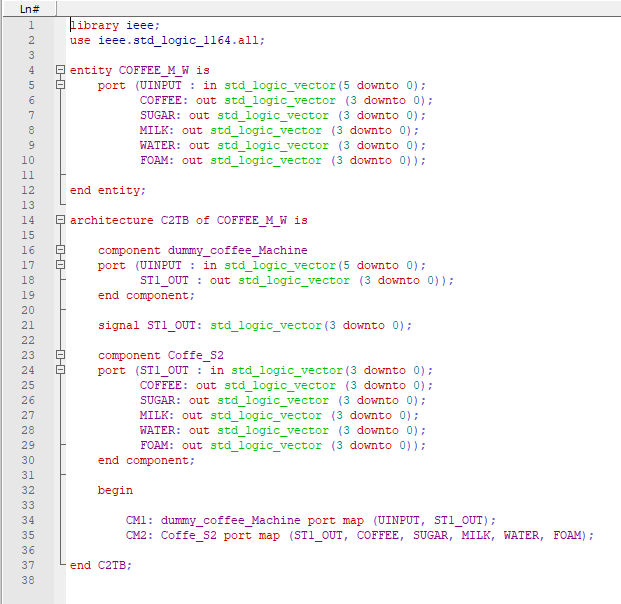
\includegraphics[scale=0.77]{imgs/vhdl3}}
\caption{Third VHDL module}
\label{fig:vhdl3}
\end{figure}

Finally we wrote test benches for each one of the modules to check that the behaviour was as expected. in Figure \ref{fig:tb1} we have an example of the test bench.

\begin{figure}[H]
\centering{ 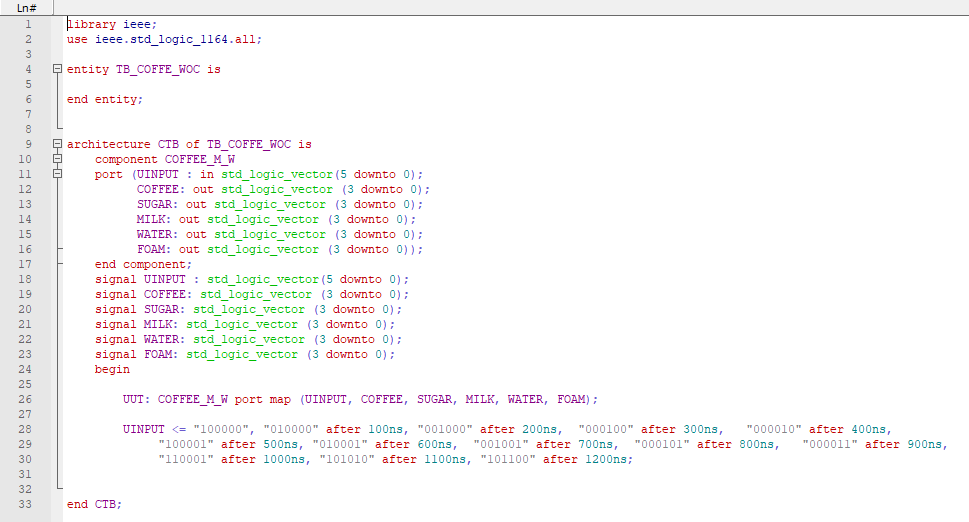
\includegraphics[scale=0.6]{imgs/tb1}}
\caption{Test bench}
\label{fig:tb1}
\end{figure}

\subsection{PCB Design}

\subsubsection{Xilinx}

The process of design of PCB started with the programming started with ModelSim with the design and simulation of the VHDL code and ends in Xilinx-ISE with the design of the FPGA. 

In our scenario the process was as follows:

  
\begin{figure}[!h]
\centering{ 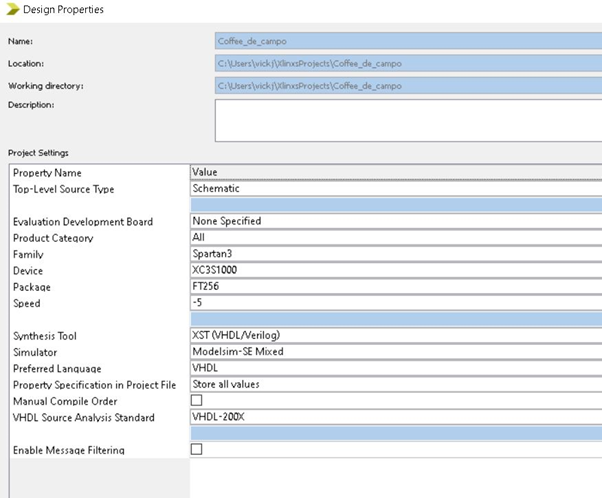
\includegraphics[scale=0.8]{imgs/xil1}}
\caption{Xilinx-ISE Design Properties}
\label{fig:xil1}
\end{figure}

\begin{enumerate}
  \item Creation of Project: To start a new project in Xilinx-ISE where you will have to input all the design properties such as family etc. In our case, the following was our unique properties are outlined in the Figure \ref{fig:xil1}. 

  
  These properties are important because they will help in determining how the system would work. 
  
  \item Check Syntax: This is done to confirm that the syntax of the VHDL code is correct and it won't throw up an error during the course of synthesis.
  
  \item Synthesize-XST: This is important to be able to generate the schematics. After this has been run, two sets of schematics are generated: RTL Schematics (This is the general schematics that can be applied to any FPGA) and Technology Schematics which is applied to a particular device configured, in our case Spartan3.
  
\begin{figure}[H]
\centering{ 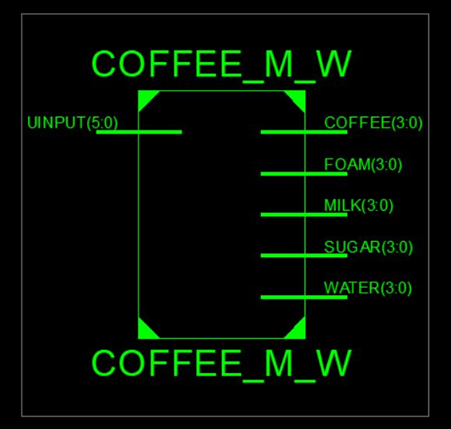
\includegraphics[scale=0.8]{imgs/xil2}}
\caption{RTL Schematics 1}
\label{fig:xil2}
\end{figure}
  
\begin{figure}[H]
\centering{ 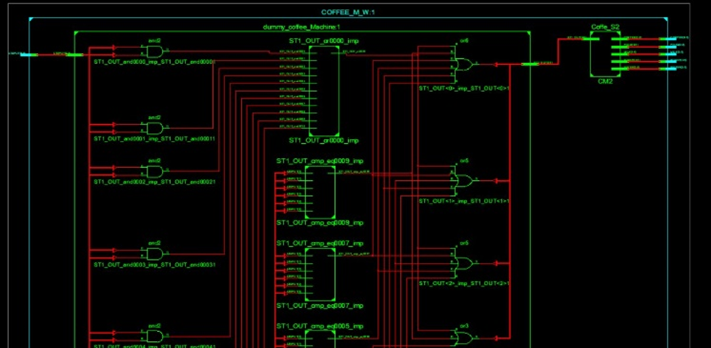
\includegraphics[scale=0.8]{imgs/xil3}}
\caption{RTL Schematics 2}
\label{fig:xil3}
\end{figure}  

\begin{figure}[H]
\centering{ 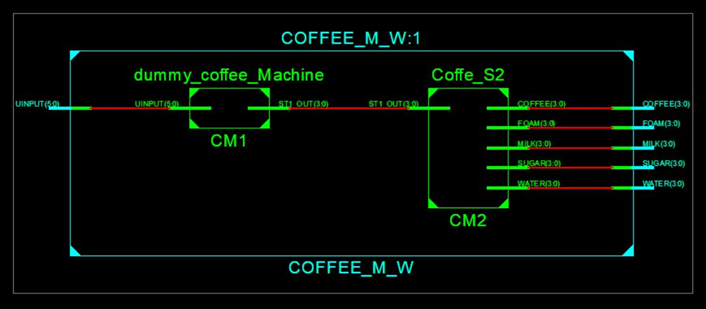
\includegraphics[scale=0.8]{imgs/xil4}}
\caption{RTL Schematics 3}
\label{fig:xil4}
\end{figure}
 
\begin{figure}[H]
\centering{ 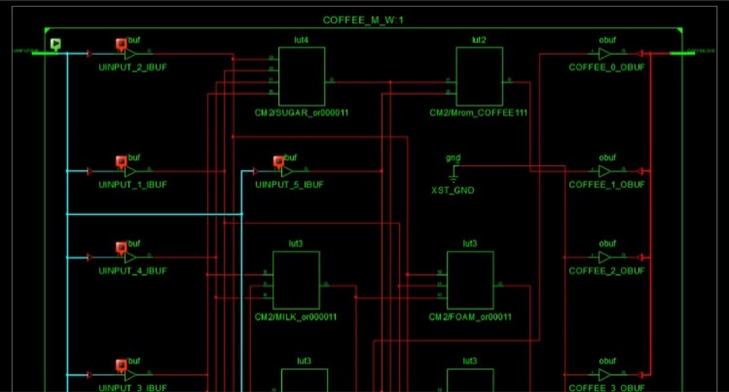
\includegraphics[scale=0.7]{imgs/xil5}}
\caption{Technology Schematics }
\label{fig:xil5}
\end{figure}
 
  \item Creating the User Constraint file: The user constraint file is used to map the various input and outputs of the device to the pins of the FPGA. The right pin is seen in the documentation of the FPGA. Figure \ref{fig:xil6}  
  
\begin{figure}[H]
\centering{ 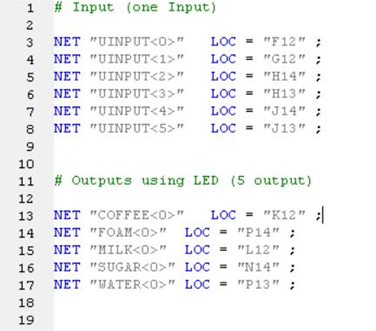
\includegraphics[scale=0.6]{imgs/xil6}}
\caption{User constraint file}
\label{fig:xil6}
\end{figure}  
  
  \item Implement Design: This was the final step of our FPGA design/ programming, such that it was used to generate the actual design and map the various FPGA pins. The diagram confirms how it will appear with the board and how we can easily interact with it. Figures \ref{fig:xil8}, \ref{fig:xil9}, \ref{fig:xil10} and \ref{fig:xil11} shows scans from the result generated.  
  
\begin{figure}[H]
\centering{ 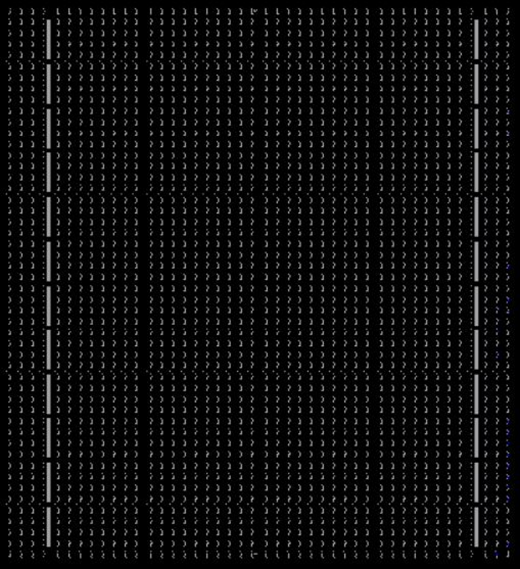
\includegraphics[scale=0.5]{imgs/xil7}}
\caption{Implement design 1}
\label{fig:xil7}
\end{figure}  

\begin{figure}[H]
\centering{ 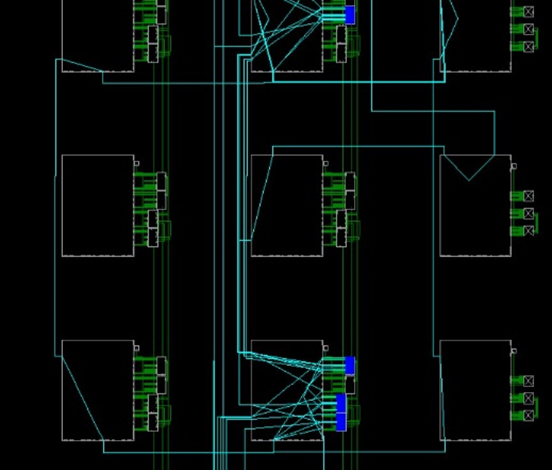
\includegraphics[scale=0.7]{imgs/xil8}}
\caption{Implement design 2}
\label{fig:xil8}
\end{figure}  

\begin{figure}[H]
\centering{ 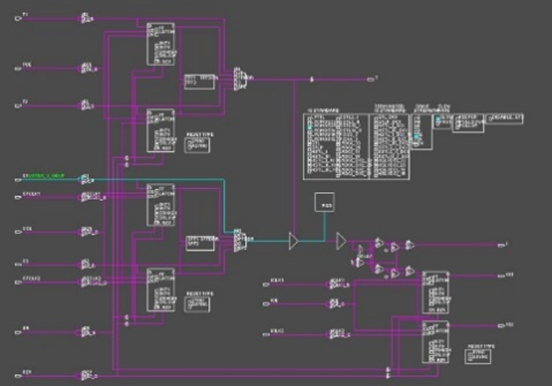
\includegraphics[scale=0.7]{imgs/xil9}}
\caption{Implement design 3}
\label{fig:xil9}
\end{figure}  

\begin{figure}[H]
\centering{ 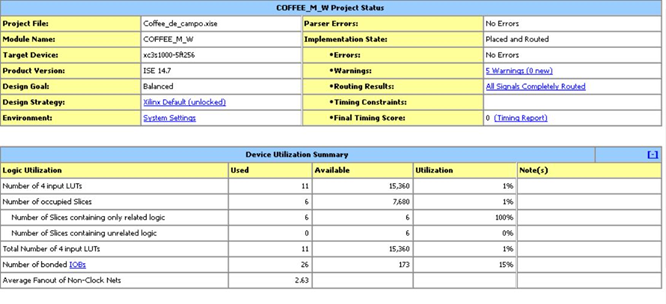
\includegraphics[scale=0.8]{imgs/xil10}}
\caption{Design Summary 1}
\label{fig:xil10}
\end{figure}  
 
\begin{figure}[H]
\centering{ 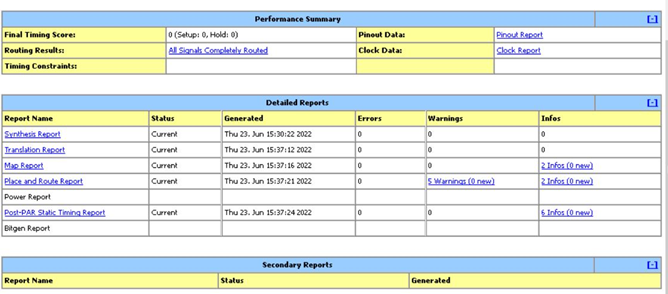
\includegraphics[scale=0.8]{imgs/xil11}}
\caption{Design Summary 2}
\label{fig:xil11}
\end{figure} 
 
\end{enumerate}

\subsubsection{Eagle}

As discussed before, in this course we were presented an opportunity to design a coffee machine using VHDL (Modelsim), FPGA (Xilings and Eagle). While the rest of the topic goes in depth, the eagle PCB design presents more of an abstract version of the project. Which we will discuss systematically in this section.

From the very beginning right after we open the software we had to create a project. In the project, we had to create a schematic file, which will allow us to create a schematic for the project that can be used later on for layout purpose, Figure \ref{fig:eagle1}.

\begin{figure}[H]
\centering{ 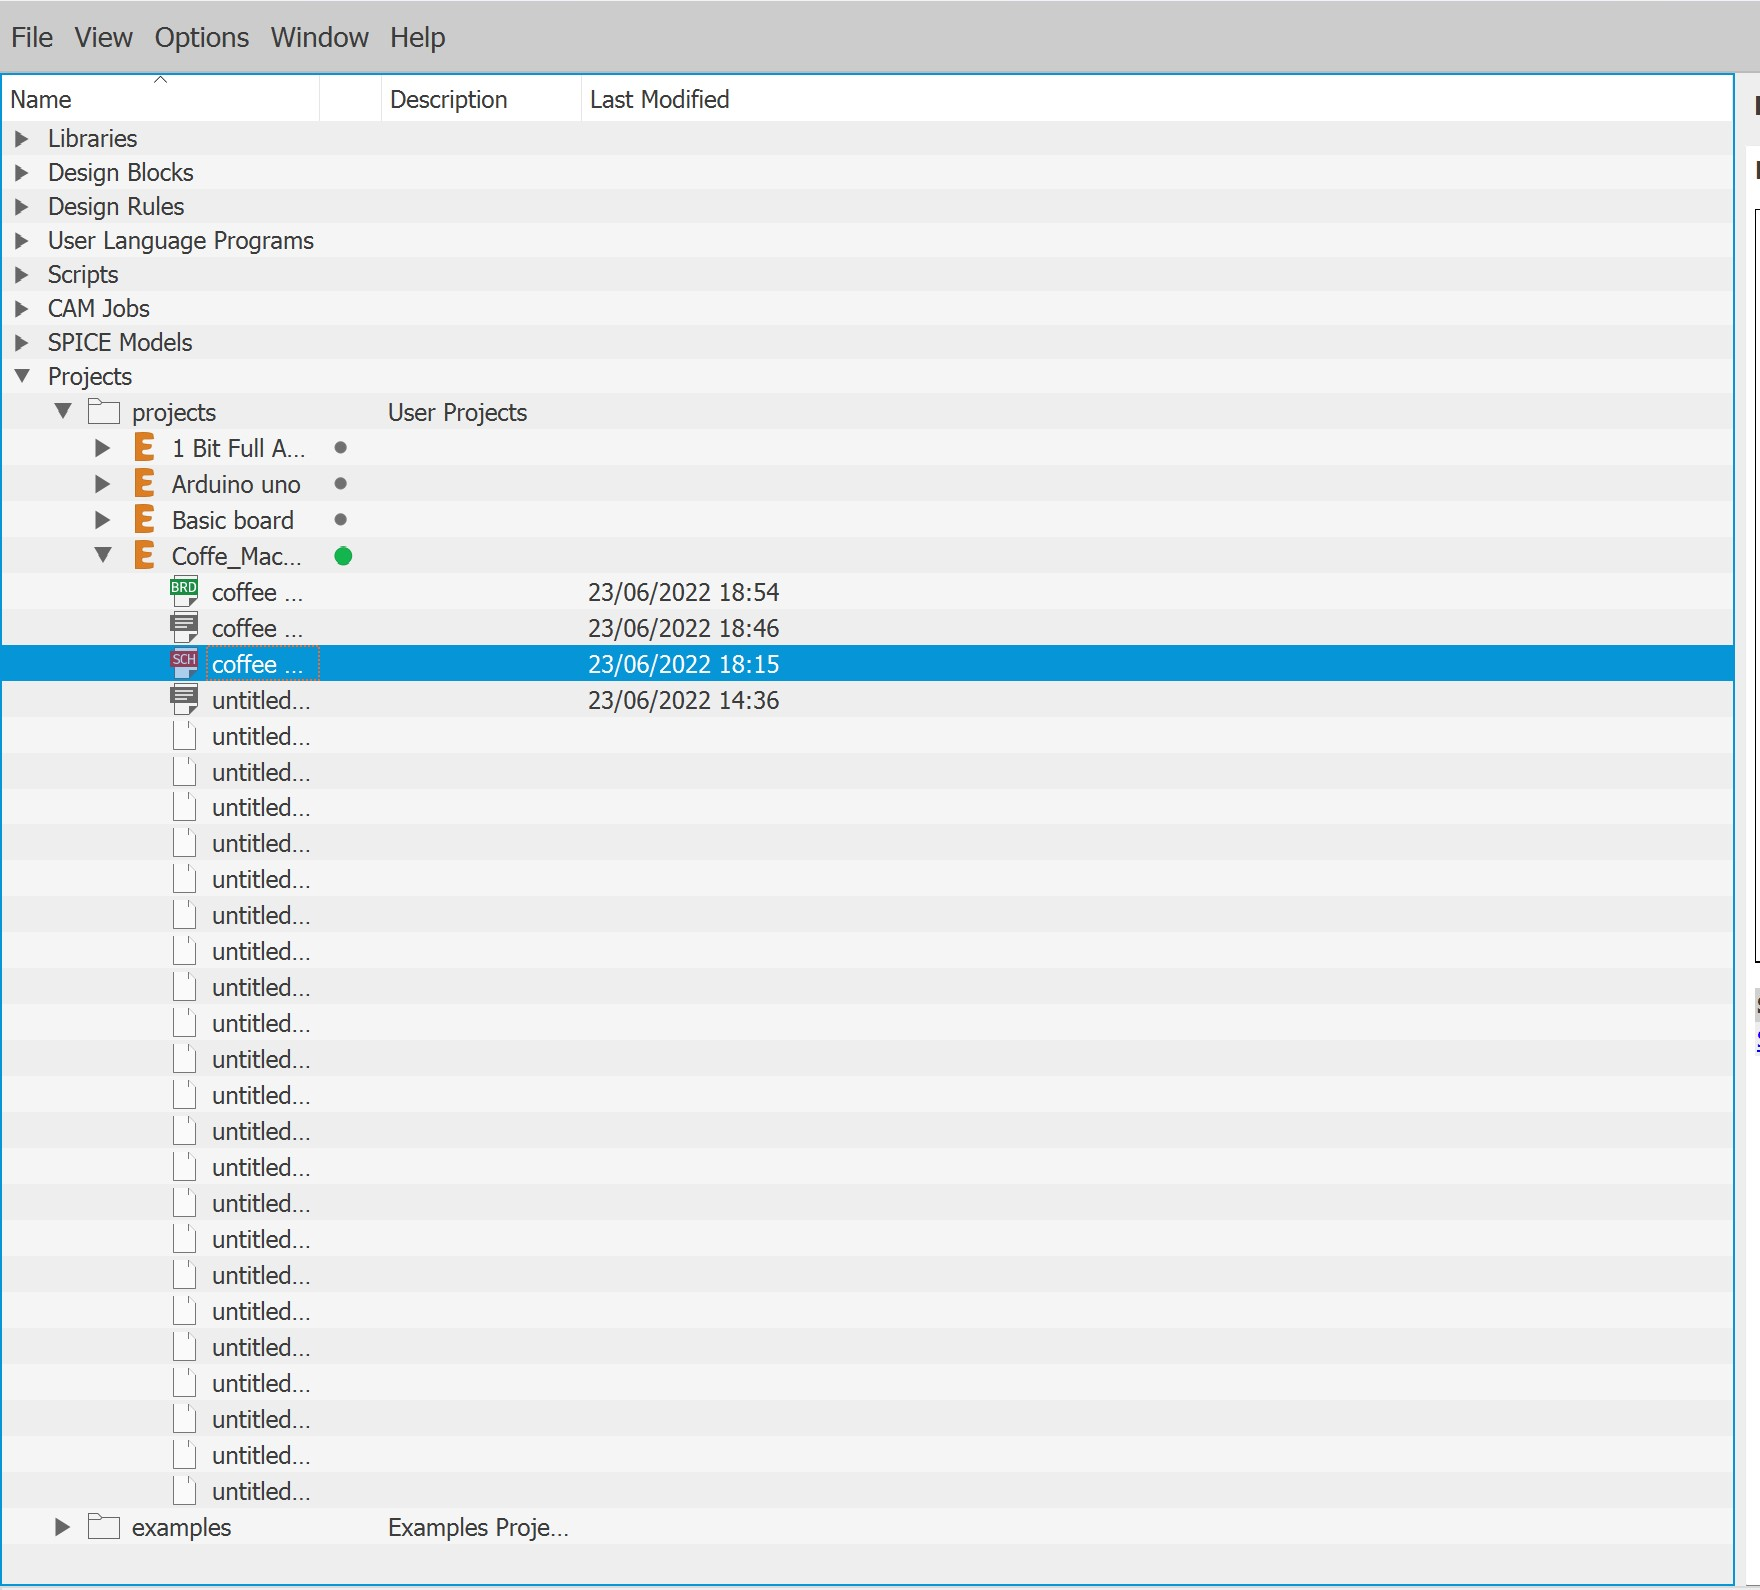
\includegraphics[scale=0.5]{imgs/Project_Pannel}}
\caption{Creating Project and Schematic}
\label{fig:eagle1}
\end{figure}

Once we created the schematic, we can now add component as necessary. To represent the button designated to the coffee we add a SWITCH- \_PUSHBUTTON component From Adafruit library which we were advised to install during our lab period along with SparkFun. Since we have five different kinds of coffee, we added 5 SWITCH\_PUSHBUTTON Designated with the name and the number of the drinks like:

\begin{enumerate}

	\item ESPRESSO
	\item AMERICANO
	\item CAPPUCCINO
	\item LATTE
	\item MACCHIATO


\end{enumerate}

and an extra button for adding sugar (6. SUGAR) Figure \ref{fig:eagle2}

\begin{figure}[H]
\centering{ 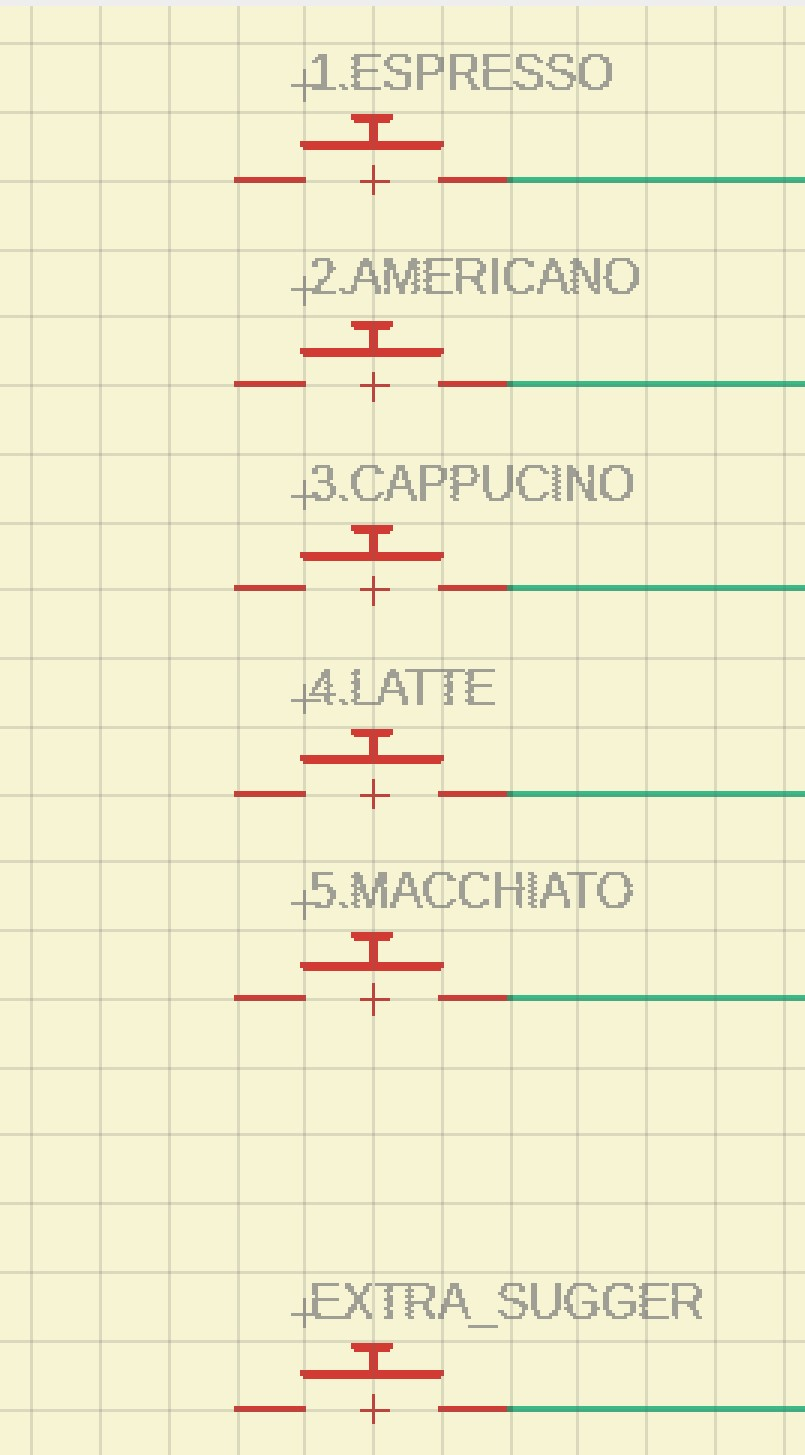
\includegraphics[scale=0.5]{imgs/button}}
\caption{Button for coffee}
\label{fig:eagle2}
\end{figure}


Since we have the necessary input now we need a microcontroller to process the algorithm for making the coffee. Therefor we choose Arduino uno r3 among many. Shown in the Figure \ref{fig:eagle3}

\begin{figure}[H]
\centering{ \includegraphics[scale=0.5]{imgs/arduinor3}}
\caption{Arduino uno}
\label{fig:eagle3}
\end{figure}


Now we need the last component to proceed to the next step. The final component will be something that shows the output for our coffee machine. And to show the output we choose LED as our component. After adding the LED and resister to our schematic, we labeled it as our five output (Fig \ref{fig:eagle4}):  \\

	1.COFFEE

	2.MILK

	3.WATER

	4.FOAM

	5.SUGAR\\
	

\begin{figure}[H]
\centering{ 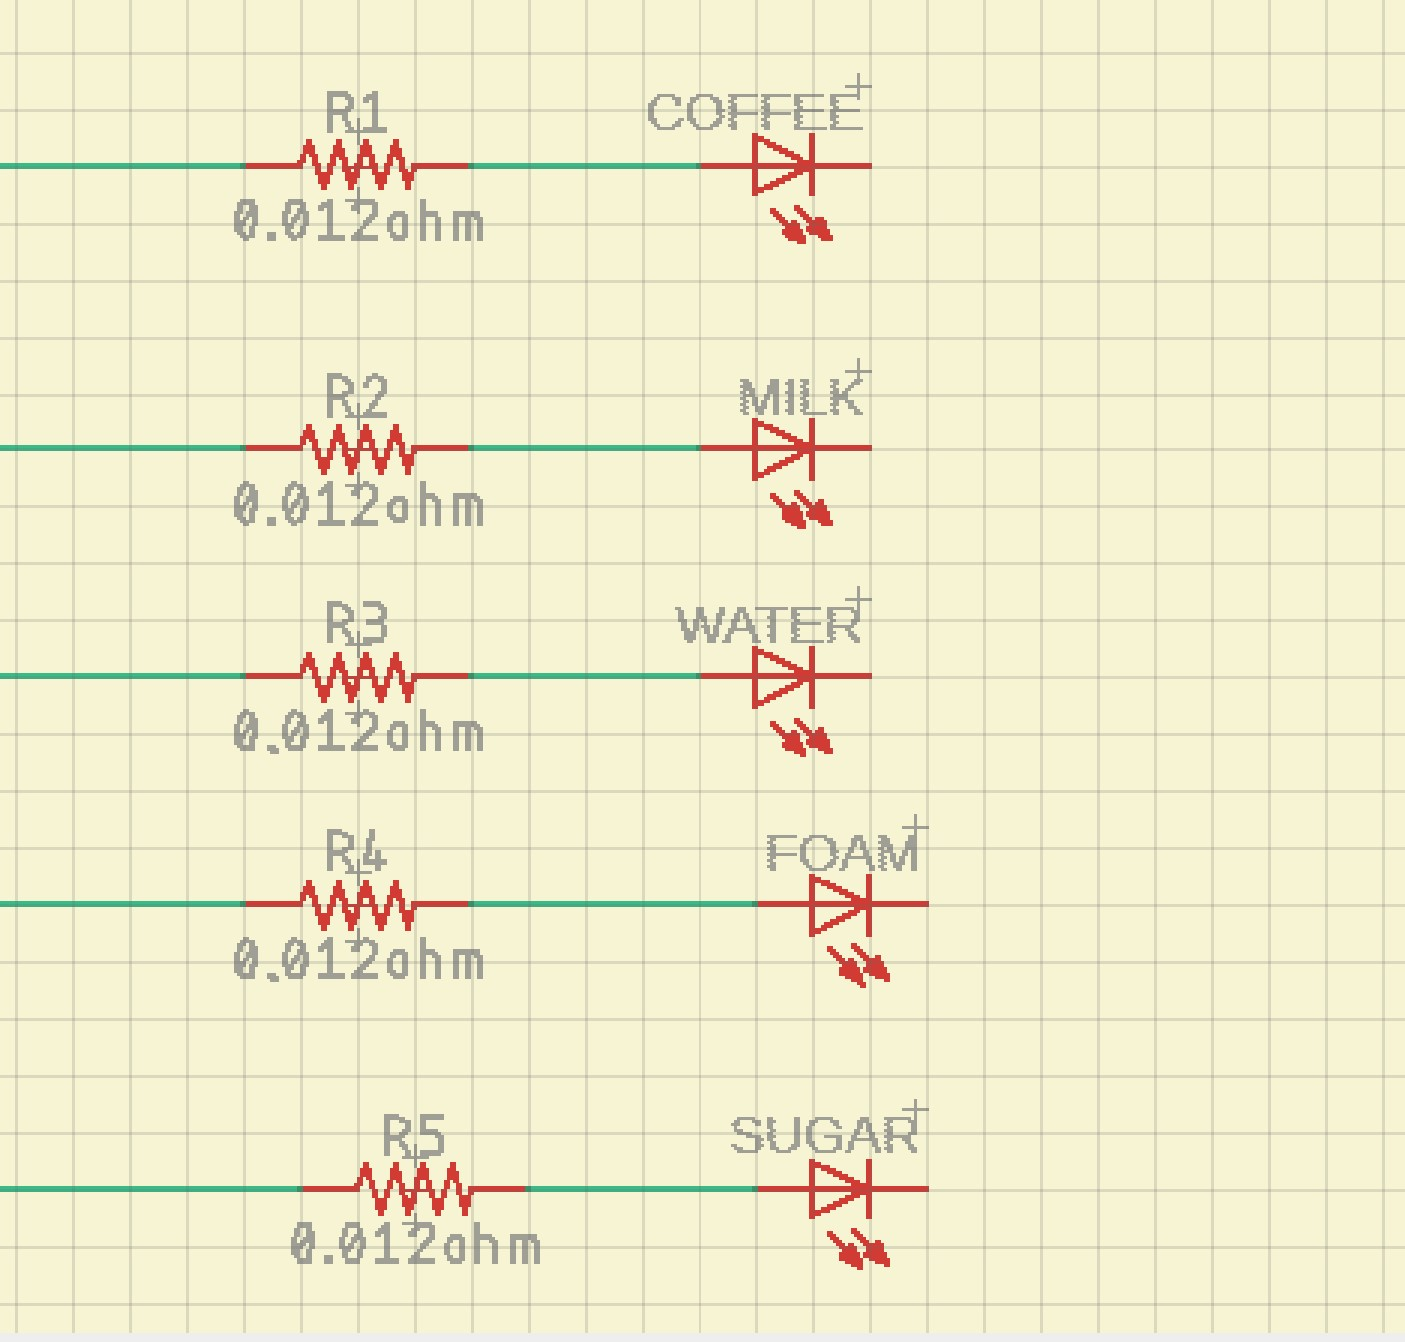
\includegraphics[scale=0.5]{imgs/led}}
\caption{Leds and resistors}
\label{fig:eagle4}
\end{figure}

Since we have all the required components, we can start to wire them together. To wire them we have to use net tool from the tool bar. In addition, for the connection we wire the ports as shown on the table, as well as in the Figure \ref{fig:eagle5} \\



Input:			

1. ESPRESSO          to D13 

2.AMERICANO       to 12		

3.CAPPUCINO        to D11		

4.LATTE                   to D10		

5.MACCHIATO        to D9			

6. EXTRA\_SUGAR   to D8  \\

 
Output:

1.COFFE	to D3

			  2.MILK	to D4

			  3.WATER	to D5

			  4.FOAM	to D6

				  5.SUGAR	to D7


\begin{figure}[H]
\centering{ 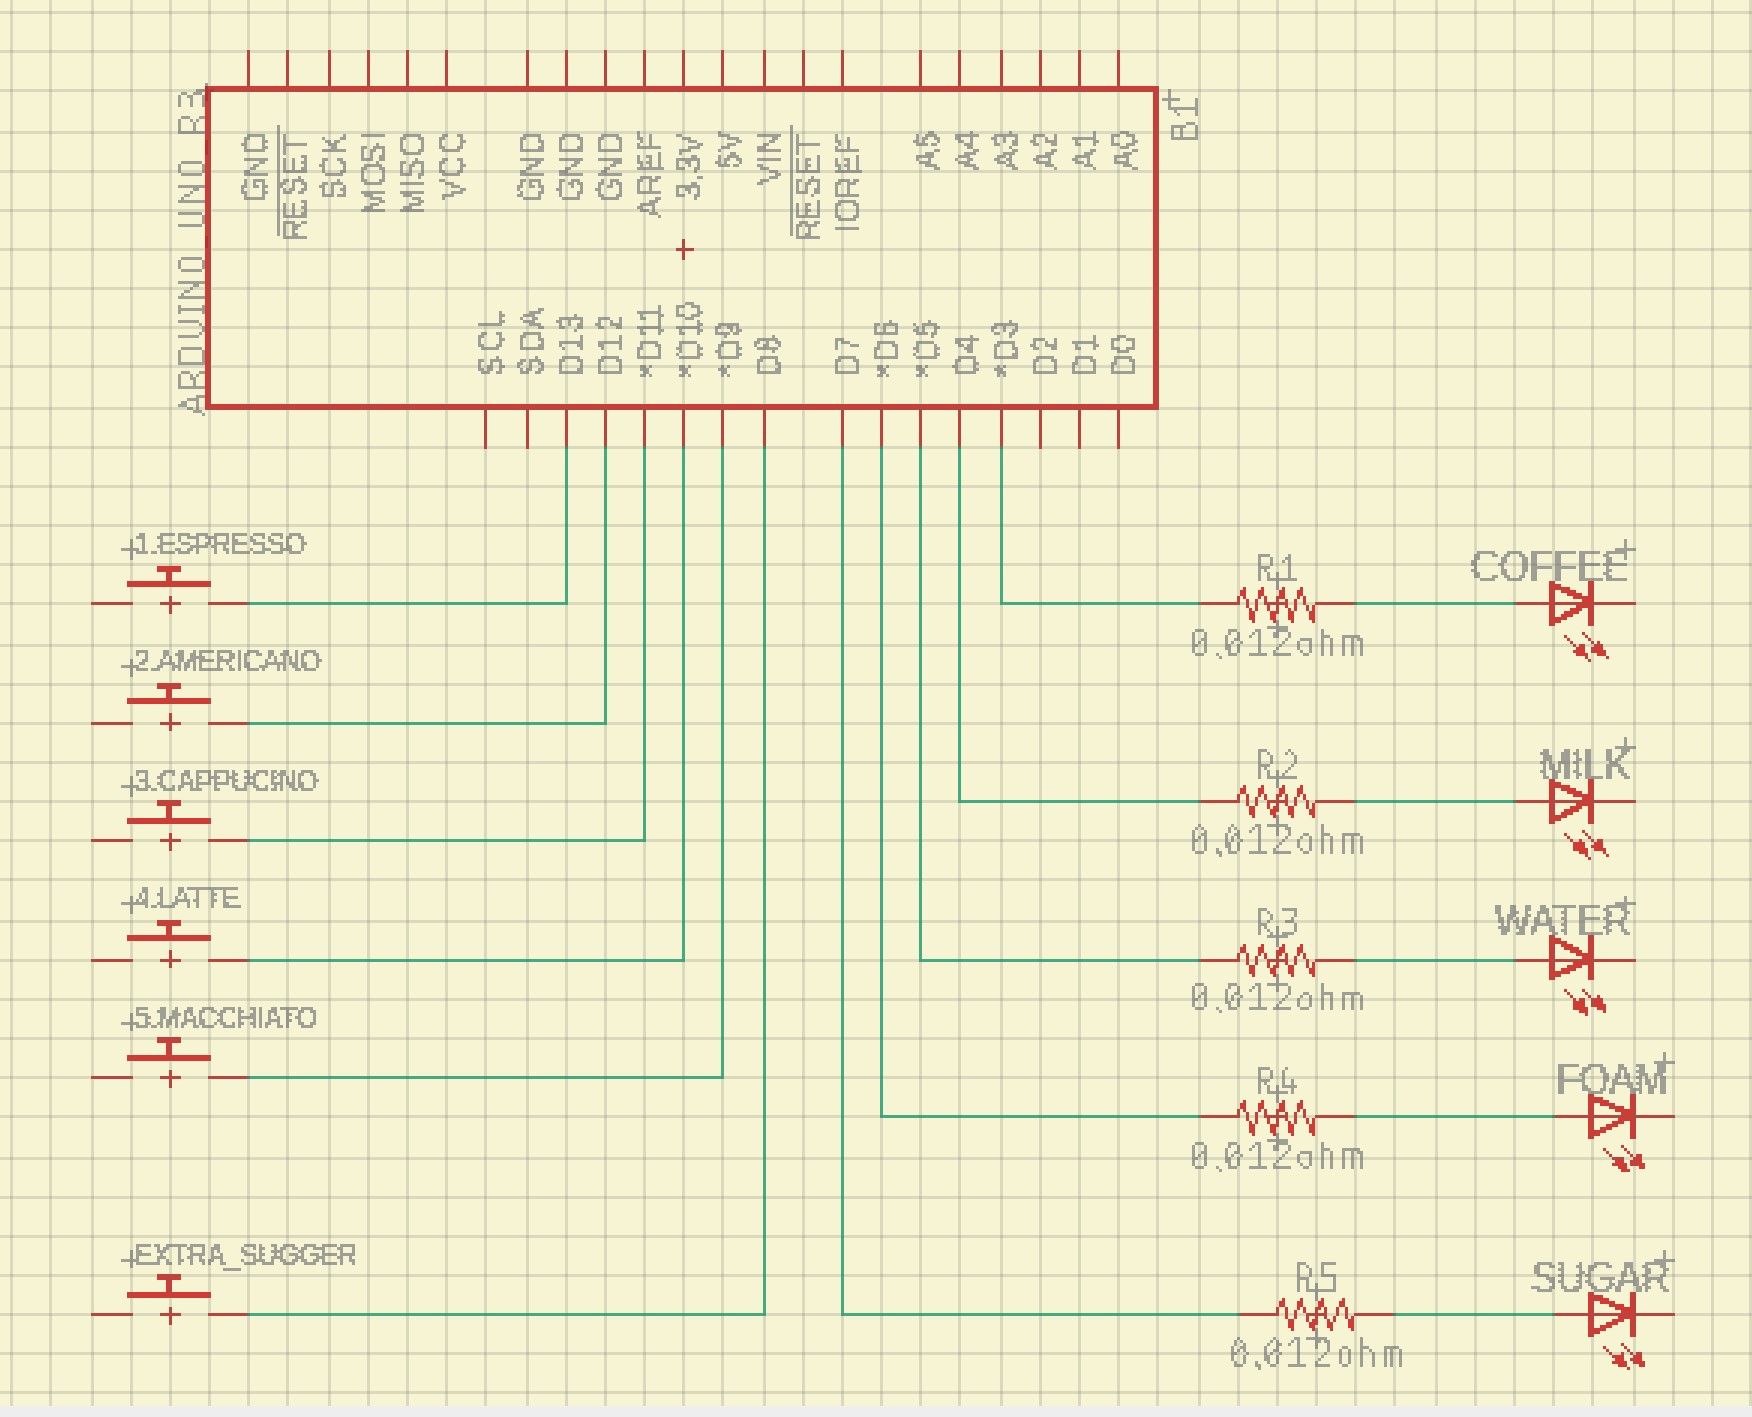
\includegraphics[scale=0.5]{imgs/whole}}
\caption{System connections}
\label{fig:eagle5}
\end{figure}

Once we are done with our schematic, we can start the layout process. Since our project is a simple one, we chose single one-sided layer to put out components on the board.
We could jump to the layout section. Once we are in the layout window we can start mapping out component such a way that it reduce better prevent cross wiring and clutter. For that we did the component placement manually and for wiring we used auto command. Using auto command, it reduce the workload a lot. Once the process is done then we start to manually correct the wiring as necessary. Some time moving the wires or component and sometime rotating the component, either way which ever provides the best outcome. The Layout can be seen from the Figure \ref{fig:eagle6}.

\begin{figure}[H]
\centering{ 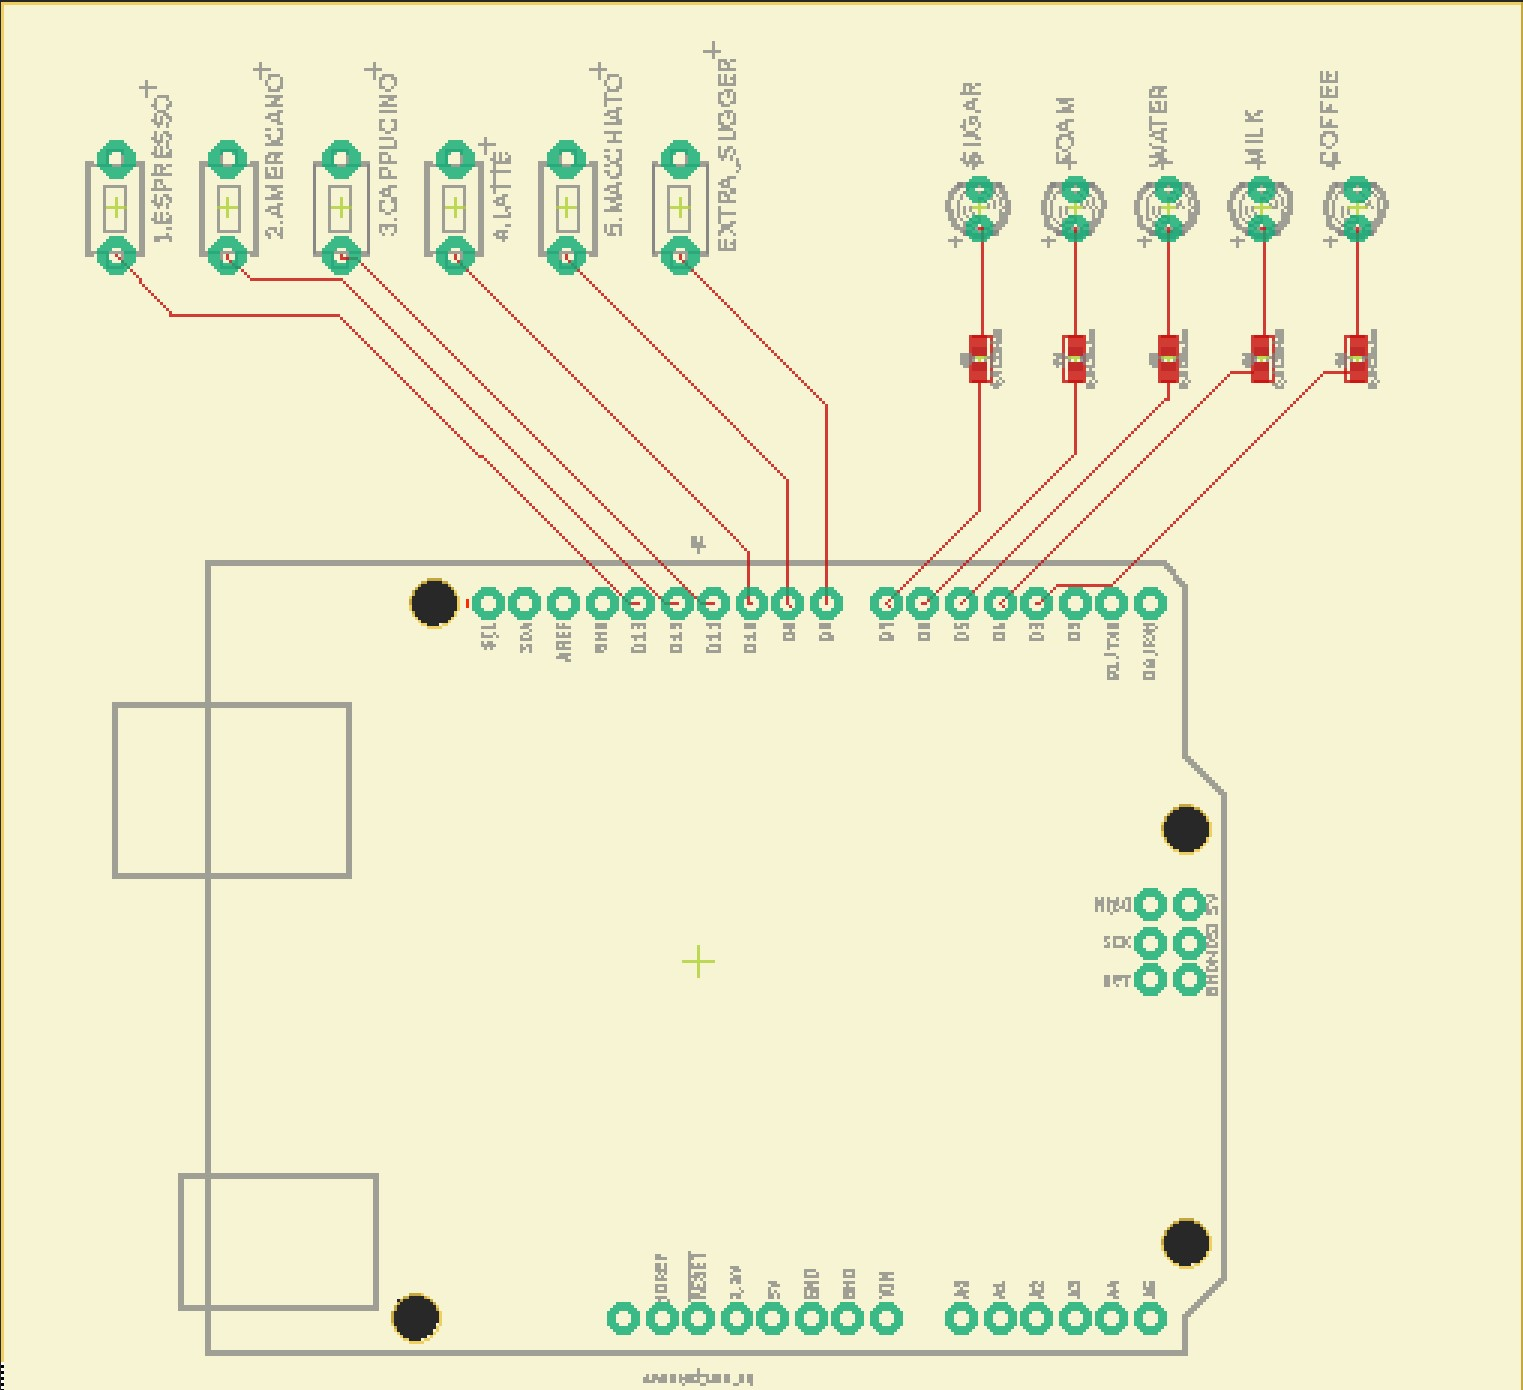
\includegraphics[scale=0.5]{imgs/layout}}
\caption{Layout of Café Del Campo}
\label{fig:eagle6}
\end{figure}

By following the steps from schematic to layout we were able to achieve the Café del campo using AutoDesk Eagle.


\newpage

\begin{thebibliography}{9}
\bibitem{kanvanize}
Kanvanize. (n.d.). What Is Agile Project Management? A Comprehensive Guide. Kanban Software for Agile Project Management. https://kanbanize.com/agile/project-management

\bibitem{APM}
APM. (n.d.). Agile project management. What Is Agile Project Management? https://www.apm.org.uk/resources/find-a-resource/agile-project-management/

\bibitem{APM1}
APM. (n.d.-b). What is project management? https://www.apm.org.uk/resources/what-is-project-management/

\bibitem {github}
GitHub. (n.d.). About projects. About Projects. https://docs.github.com/en/issues/trying-out-the-new-projects-experience/about-projects

\bibitem {fpga}
Palanisamy, R., Boopathi, C. S., Selvakumar, K., and Vijayakumar, K. (2020). Switching pulse generation for DC-DC boost converter using Xilinx-ISE with FPGA processor. International Journal of Electrical and Computer Engineering, 10(2), 1722.

\bibitem{eagle}
Wikipedia contributors. (2022, February 1). EAGLE (program). Wikipedia. https://en.wikipedia.org/wiki/EAGLE\_(program)

\bibitem{vhdl}
Navabi, Z. (1993). VHDL: Analysis and modeling of digital systems (Vol. 2). New York: McGraw-Hill.

\end{thebibliography}

\end{document}